\let\negmedspace\undefined
\let\negthickspace\undefined
\documentclass[journal,12pt,twocolumn]{IEEEtran}
\usepackage{cite}
\usepackage{amsmath,amssymb,amsfonts,amsthm}
\usepackage{algorithmic}
\usepackage{graphicx}
\usepackage{textcomp}
\usepackage{xcolor}
\usepackage{txfonts}
\usepackage{listings}
\usepackage{enumitem}
\usepackage{mathtools}
\usepackage{gensymb}
\usepackage[breaklinks=true]{hyperref}
\usepackage{tkz-euclide} % loads  TikZ and tkz-base
\usepackage{listings}
\usepackage{gvv}
\newtheorem{theorem}{Theorem}[section]
\newtheorem{problem}{Problem}
\newtheorem{proposition}{Proposition}[section]
\newtheorem{lemma}{Lemma}[section]
\newtheorem{corollary}[theorem]{Corollary}
\newtheorem{example}{Example}[section]
\newtheorem{definition}[problem]{Definition}
%\newtheorem{thm}{Theorem}[section] 
%\newtheorem{defn}[thm]{Definition}
%\newtheorem{algorithm}{Algorithm}[section]
%\newtheorem{cor}{Corollary}
\newcommand{\BEQA}{\begin{eqnarray}}
\newcommand{\EEQA}{\end{eqnarray}}
\newcommand{\define}{\stackrel{\triangle}{=}}
\theoremstyle{remark}
\newtheorem{rem}{Remark}

%\bibliographystyle{ieeetr}
\begin{document}
%

\bibliographystyle{IEEEtran}


\vspace{3cm}

\title{
%  \logo{
Assignment-2

\large{EE:1205 \brak{Signals  Systems}}

Indian Institute of Technology, Hyderabad
%  }
}
\author{Md Ayaan Ashraf

EE23BTECH11041
}  
\maketitle
\newpage
\bigskip
\renewcommand{\thefigure}{\theenumi}
\renewcommand{\thetable}{\theenumi}
%\renewcommand{\theequation}{\theenumi}
\section*{\textit{\textbf{Question 11.9.3.22}}}
 If the first and the nth term of a G.P. are a and b, respectively, and if P is the product of n terms , prove that $ P^2 = \brak{ab}^n $
\section*{\textit{\textbf{Solution:}}}

\begin{table}[ht]
  \centering
  \begin{tabular}{|c||c||c|}
    \hline
      Parameter & Value & Description  \\
    \hline
       $x(0)$ & a & First Term\\
     \hline
      $r$ & ? & Common Ratio \\
    \hline
    $x(n)$ & b & $n^{th}$ term\\
    \hline
     P & ? & Product of n terms\\
     \hline
  \end{tabular}
  \vspace{2mm}
  \caption{Parameter Table 11.9.3.22}
\end{table}`

\begin{align}
x\brak{n} = & x\brak{0}r^{n} \brak{u\brak{n}}\\
\brak{x\brak{0}x\brak{n}}^n = & \brak{x\brak{0}}^{2n} r^{n^2}\\
P =& \prod_{k=0}^{n} x\brak{0}r^{k}= \brak{x\brak{0}}^n r^{\frac{n^2}{2}}\\
P^2 =& \brak{x\brak{0}}^{2n} r^{n^2}
\end{align}
\\
From \brak{2} and \brak{4} , $ P^2 = \brak{x\brak{0}x\brak{n}}^n $\\
\\
Z-transform of x\brak{n}:
\begin{align}
X\brak{z}= \frac{x\brak{0}}{1-rz^{-1}} , \quad{|z|>r}
\end{align}
\begin{figure}[ht]
    \centering
    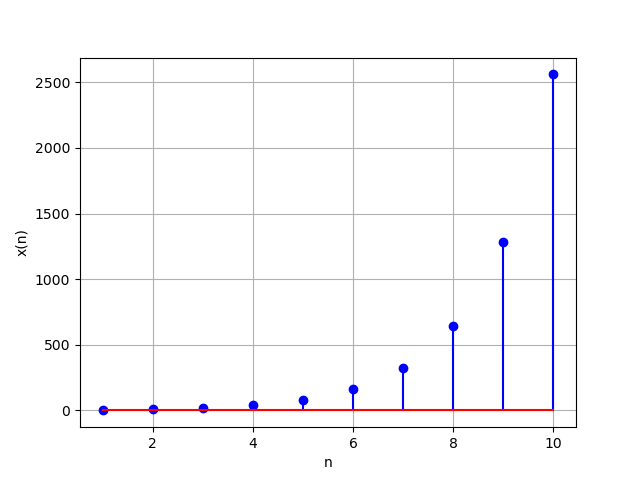
\includegraphics[width=\columnwidth]{figs/fig.png}
    \caption{Plot of x\brak{n}= $\brak{5}\brak{2}^n$}
    \label{fig: 11.9.3.22}
\end{figure}
\end{document}
